
Nuestro algoritmo como mencionamos anteriormente presenta dos ciclos predominantes de los cuales el segundo ciclo es el que realiza la busqueda de las pesas.\\

El primero ciclo consta en armar un arreglo de sumas de potencias de tres $sumasParciales$, donde la $i-esima$ posición es la suma desde $3^0$ hasta $3^i$ y la $n-esima$ será la suma desde $3^0$ hasta $3^n$  tal que es igual a $P$ o en su defecto el inmediato mayor. 

Podemos notar que para representar un número en base tres necesitamos $\ceil[\big]{log_3(P)}$ divisiones con lo que obtendremos un total de $\ceil[\big]{log_3(P)}$  potencias de tres. 
En nuestro algoritmo, puede ser necesario tomar la potencia inmediatamente mayor a $P$ por lo cual tendriamos $\ceil[\big]{log_3(P)}$ + 1 potencias de tres en el peor caso. Veamos que esto es cierto:\\

Sea $3^i \geq P  \geq 3^{i-1}$ con $(P, i) \in \mathbb{N}$.\\

Si tomamos $log_3$ a ambos lados de la desigualdad tenemos

\begin{equation}
log_3(3^i) \geq log_3(P)  \geq log_3(3^{i-1}) \iff i \geq log_3(P)  \geq i-1
\end{equation}

tomando parte entera superior nos queda:

\begin{equation}
i \geq \ceil[\big]{log_3(P)}  \geq i-1 
\end{equation}

Con lo cual tenemos que $\ceil[\big]{log_3(P)}+1  \geq i$ potencias de tres a utilizar en el peor caso. Y este será el tamaño del arreglo de $sumasParciales$.\\
 
El segundo ciclo corresponde a la resolución del algoritmo.
Se comienza con un equilibrio igual a $P$ al que nos referiremos como $equilibrioActual$ y se busca llevar este valor a cero mediante sumas o restas de potencias de tres. \\
Si el valor inicial $P$ es suma de potencias, para lograr que $equilibrioActual$ sea cero, necesitaria utilizar todas las potencias, lo cual implica usar las $\ceil[\big]{log_3(P)}+1$ que hay en el arreglo $sumasParciales$. \\
Independientemente de si lo anterior sucede o no, el arreglo $sumasParciales$ se recorre completo, es decir, las $\ceil[\big]{log_3(P)}+1$ posiciones del mismo.\\

Por lo tanto la complejidad total será:

\begin{equation}
O(2 \ast \ceil[\big]{log_3(P)} + 1) \subseteq O(\ceil[\big]{log_3(P)})
\end{equation}

Como $log_3(P)$ y $\sqrt(P)$ son funciones estrictamente crecientes y $log_3(P)$ $<$ $\sqrt(P)$ para todo entero positivo.\\

\vspace*{0.3cm} \vspace*{0.3cm}
  \begin{center}
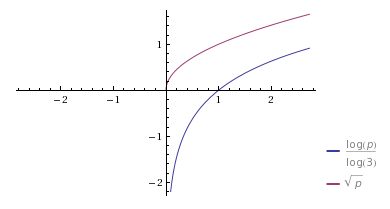
\includegraphics[scale=0.65]{./EJ2/imgpsh_fullsize.png}
  \end{center}
  \vspace*{0.3cm}
  
Podemos concluir que:\\

\begin{equation}
O(\ceil[\big]{log_3(P)}) \subseteq O(\sqrt(P))
\end{equation}
